\documentclass{standalone}
\usepackage{tikz}
\usepackage{pgfplots}
\pgfplotsset{compat=newest}

\begin{document}

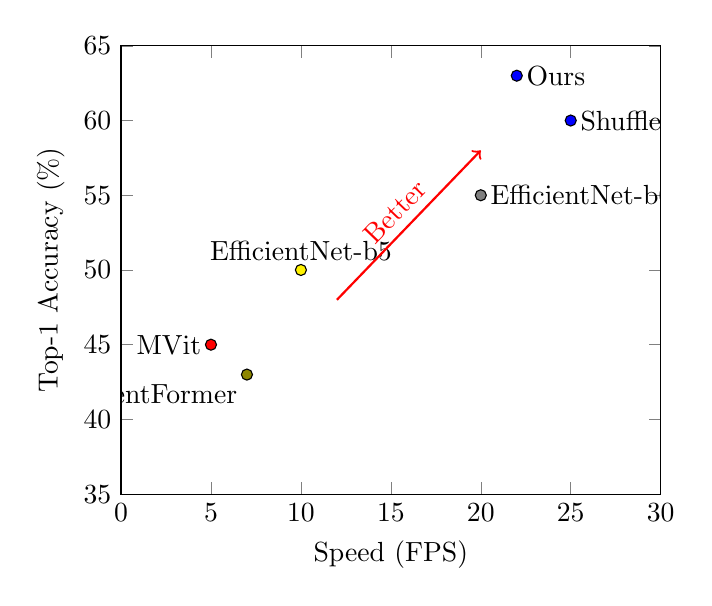
\begin{tikzpicture}

    \begin{axis}[
        xlabel={Speed (FPS)},
        ylabel={Top-1 Accuracy (\%)},
        xmin=0, xmax=30,
        ymin=35, ymax=65,
        xtick={0, 5, 10, 15, 20, 25, 30},
        ytick={35, 40, 45, 50, 55, 60, 65},
        scatter/classes={
            a={mark=*,draw=black,fill=red},
            b={mark=*,draw=black,fill=yellow},
            c={mark=*,draw=black,fill=gray},
            d={mark=*,draw=black,fill=olive},
            e={mark=*,draw=black,fill=blue}
        },
        scatter,
        only marks,
        point meta=explicit symbolic,
    ]

    \addplot[scatter,only marks,scatter src=explicit symbolic]
    coordinates {
        (5,45) [a]
        (10,50) [b]
        (20,55) [c]
        (7,43) [d]
        (25,60) [e]
        (22,63) [e]
    };

    \node[anchor=east] at (axis cs:5,45) {MVit};
    \node[anchor=south] at (axis cs:10,50) {EfficientNet-b5};
    \node[anchor=west] at (axis cs:20,55) {EfficientNet-b0};
    \node[anchor=north east] at (axis cs:7,43) {EfficientFormer};
    \node[anchor=west] at (axis cs:25,60) {ShuffleNetV2};
    \node[anchor=west] at (axis cs:22,63) {Ours};

    \draw[->, red, thick] (axis cs:12,48) -- (axis cs:20,58) node[midway, above, sloped] {Better};

    \end{axis}

\end{tikzpicture}

\end{document}